\section{Theoretische Grundlagen}
\label{sec:theorie}

Grundlage für den Versuch stellte die Wärmeübertragung am Rohr da. So lässt sich der übertragende Wärmestrom über die spezifische Wärmekapazität, dem Massenstrom, sowie aus der Differenz zwischen eingehender und ausgehender Temperatur des Stromes.
\begin{flalign}
 	\dot{Q} &= \dot{m}*c_p*\Delta T\\
 	\dot{Q} &= \dot{m}*c_p*(T_\omega-T_\alpha)
\end{flalign}
Da für die eigentliche Wärmeübertragung in Wärmetauschern oft keine konstante Temperaturdifferenz vorliegt, verwendet man für die Berechnung des Wärmedurchgangskoeffizienten, mit der Fläche des Wärmetauschers, gern die logarithmische Temperaturdifferenz. Mit dem zuvor berechneten Wärmestrom lässt sich so $U_a$ ausrechnen.
\begin{flalign}
	\Delta T_{_{\ln}}	&=  \frac{\Delta T_A-\Delta T_B}{\ln\left(\frac{\Delta T_A}{\Delta T_B}\right)}\\[1mm]
	\dot{Q} 	 &= U_a *A*\Delta T_{_{\ln}}\\
	U_a				&= \frac{\dot{Q}}{\Delta T_{_{\ln}}}
\end{flalign}
Für die weitere Charakterisierung der Strömung außerhalb des Rohrs wird der hydraulische Rohrdurchmesser $d_H$ als theoretische Größe eingeführt. Er soll sicherstellen, dass die vorherrschenden, turbulenten Strömungen ändernd gut beschrieben werden können.
\begin{flalign}
	d_H \, (\text{Rohr})	&= D_i-d_a
\end{flalign}
Solche Größen sind unter anderem die Reynoldszahl $Re$ zur Charakterisierung der Strömung als turbulent, laminar oder einem Übergangszustand.
\begin{flalign}
	Re	&= \frac{d*w}{\nu}
\end{flalign}
Die Prandtl-Zahl hingegen gibt das Verhältnis zwischen kinematischer Viskosität $\nu$ und der Temperaturleitfähigkeit $a$ an.
\begin{flalign}
		Pr	&= \frac{c_p*\nu*\rho}{\lambda}
\end{flalign}
Idealer Weise lässt sich so aus den beiden zuletzt genannten Größe eine weitere, neue, dimensionslose Kennzahl definieren um den konvektiven Wärmeübergang zwischen einer festen Oberfläche und einem strömenden Fluid zu beschreiben. Die \textsc{Nußelt}-Zahl $Nu$. Für die äußere Wasserströmung lässt sich dieser Übergang als ideal annehmen, da der Wärmeübergang der Luft deutlich stärker die Übertragung beeinflusst.
\begin{flalign}
	Nu_{\text{ideal}}	&= 0,023*\left(Re^2*Pr\right)^{0,4}
\end{flalign}
Aus einem weiteren Zusammenhang der \textsc{Nußelt}-Zahl gegenüber der Wärmekonvektion, lässt sich so der Wärmeübergangkoeffizient $\alpha_a$ für die wasserseitige Wärmeübertragung berechnen.
\begin{flalign}
	Nu 	&= \frac{\alpha*d}{\lambda}\\[1mm]
	\alpha	&=  \frac{Nu*\lambda}{d}
\end{flalign}
Unter diesen Annahmen ist es nun so auch möglich mit Hilfe des Wärmeleitwiderstandes, der geometrischen Daten der Rohre, des Wärmedurchgangskoeffizientens und des Wärmeübergangskoeffizienten des Wassers (außen), der Wärmeübergangskoeffizient der Luft zu berechnen.
\begin{flalign}
U_a		&=\left(\frac{d_a}{\alpha_i*d_i}+\frac{d_a}{2*\lambda}*\ln\left[\frac{d_a}{d_i}\right]+\frac{1}{\alpha_a}\right)^{-1}\\[1mm]
\alpha_i&= \left[\left(\frac{1}{U_a}-\frac{d_a}{2*\lambda}*\ln\left[\frac{d_a}{d_i}\right]-\frac{1}{\alpha_a}\right)*\frac{d_i}{d_a}\right]^{-1}
\end{flalign}
Über die \textsc{Nußelt}-Zahl lässt sich dann wiederum die \textsc{Nußelt}-Zahl der  Luftseite berechnen, welche die \textsc{Nußelt}-Koeffizienten $a$ und $b$ zur Bewertung der Versuchsrohre bzw. der Strömungsgeschwindigkeiten einschätzen lässt.
\begin{flalign}
	a	&= e^{\ln(Nu)}
\end{flalign}
\begin{flalign}
	b &= f'\left(\ln(Re^2*Pr),\ln(Nu)\right)
\end{flalign}

Im Folgenden sind die genutzten geometrischen Rohrdaten, sowie die Stoffdaten hinterlegt.

\begin{table}[h!]
	\centering
	\caption{Rohrdaten}
	\label{tab:rohrdaten}%
	\renewcommand{\arraystretch}{1.2}
	%\resizebox{14cm}{!}{
		\begin{tabulary}{1.15\textwidth}{C|CCC}
			\hline
			&\textbf{WÜ 1} & \textbf{WÜ 4} & \textbf{WÜ 6}\\
			\hline
			$d_i \left[\si{\milli \meter}\right]$&17,3&29,7&17,3\\
			$d_a \left[\si{\milli \meter}\right]$&21,3&33,7&21,3\\
			$D_i \left[\si{\milli \meter}\right]$&29,7&44,3&29,7\\
			$D_a \left[\si{\milli \meter}\right]$&33,7&48,3&33,7\\	
			$L \left[\si{\milli \meter}\right]$&800&800&400\\
			\hline
	\end{tabulary}
%}
\end{table}%
\FloatBarrier
\newpage
\begin{figure}[h!]
	\centering
	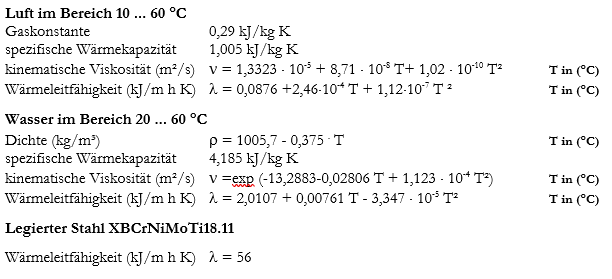
\includegraphics[width=0.9\textwidth]{img/Daten}
	\caption{Stoffdaten}
	\label{fig:stoffdaten}
\end{figure}
\FloatBarrier
%Ende


